% ============================================================================
%  Revista FARAUTE de Ciencias y Tecnología — UC/FACYT
%  Conversión a formato Faraute (guia_autor_Faraute.pdf) — cumplimiento estricto
%  Fuente: articulo_angelparejo-ITC.docx (revisado por profesores)
%  Motor: pdflatex (Times vía mathptmx). Sin biber/latexmk.
%  Compilar:  pdflatex main && pdflatex main
% ============================================================================
\documentclass[12pt,twocolumn,letterpaper]{article}

% ---- Codificación e idioma ----
\usepackage[utf8]{inputenc}
\usepackage[T1]{fontenc}
% Silabeo español vía locale ini (babel-spanish clásico no instalado).
% "Fig." y "Tabla" se re-fijan tras babel más abajo (guía Faraute).
\usepackage[spanish,provide=*]{babel}

% ---- Tipografía Times New Roman (número 12) ----
\usepackage{mathptmx}          % Times para texto y matemáticas
\usepackage[scaled=0.9]{helvet}
\usepackage{courier}
\usepackage{microtype}

% ---- Papel Carta, márgenes justificados de 2,5 cm por cada lado ----
\usepackage[letterpaper,left=2.5cm,right=2.5cm,top=2.5cm,bottom=2.5cm]{geometry}
\setlength{\columnsep}{0.7cm}

% ---- Espaciado simple ----
\usepackage{setspace}
\singlespacing

% ---- Matemáticas, tablas, figuras ----
\usepackage{amsmath,amssymb}
\usepackage{booktabs}
\usepackage{array}
\usepackage{multirow}
\usepackage{tabularx}
\usepackage{graphicx}
\usepackage[flushleft]{threeparttable}

% ---- Justificación ----
\usepackage{ragged2e}

% ---- Listas ----
\usepackage{enumitem}

% ---- Encabezados de sección: negrita y numerados (guía, punto 7) ----
\usepackage{titlesec}
\titleformat{\section}{\normalfont\bfseries}{\thesection.}{0.5em}{}
\titleformat{\subsection}{\normalfont\bfseries}{\thesubsection.}{0.5em}{}
\titlespacing*{\section}{0pt}{1.2ex plus .2ex}{0.6ex}
\titlespacing*{\subsection}{0pt}{1.0ex plus .2ex}{0.5ex}

% ---- Leyendas: "Fig." y "Tabla", tamaño 10, alineadas a la izquierda, debajo ----
\usepackage{caption}
\renewcommand{\figurename}{Fig.}
\renewcommand{\tablename}{Tabla}
\AtBeginDocument{\renewcommand{\figurename}{Fig.}\renewcommand{\tablename}{Tabla}}
\captionsetup{font=footnotesize,labelsep=period,labelfont=bf,
              justification=raggedright,singlelinecheck=false}

% ---- Enlaces ----
\usepackage[hidelinks,breaklinks]{hyperref}
\usepackage{xurl}

% ---- Numeración de ecuaciones como "Ec." al citar (guía, punto 11) ----
\newcommand{\Ec}[1]{Ec.~(\ref{#1})}

% ---- Nota de figura/tabla en tamaño 10 (Times) ----
\newcommand{\fignota}[1]{\par\vspace{2pt}\footnotesize\textbf{Nota:} #1}

\begin{document}

% ============================================================================
%  PORTADA A UNA COLUMNA: título, autores y resumen (guía, punto 2)
% ============================================================================
\twocolumn[{%
\begin{@twocolumnfalse}
\begin{center}
% ---- Título en español: Times New Roman 14, MAYÚSCULAS, negrita, centrado ----
{\fontsize{14}{17}\selectfont\bfseries
ANÁLISIS MULTICAPA DE OPERADORES DE POSTGRESQL Y ALMACENAMIENTO CSI EN KUBERNETES: UN MARCO DE ANÁLISIS Y UN ESTUDIO EMPÍRICO DE CLOUDNATIVEPG BAJO FALLOS INYECTADOS\par}

\vspace{1em}
% ---- Título en inglés: 12, negrita, iniciales mayúsculas ----
{\fontsize{12}{15}\selectfont\bfseries
Multilayer Analysis of PostgreSQL Operators and CSI Storage in Kubernetes: An Analytical Framework and an Empirical Study of CloudNativePG under Injected Faults\par}

\vspace{1.2em}
% ---- Información del autor ----
{\normalsize Angel A. Parejo R.\textsuperscript{1}\par}
\vspace{0.3em}
{\small \textsuperscript{1}Universidad de Carabobo, Valencia, Venezuela\par}
{\small angelparejo@gmail.com \quad ORCID: 0009-0001-9737-7116\par}
{\small *Autor de correspondencia: Angel A. Parejo R.; angelparejo@gmail.com\par}
\end{center}

\vspace{1em}
% ---- Resumen: máx. 150 palabras, una sola columna justificada ----
\begin{spacing}{1.0}
\noindent\textbf{Resumen.}\; \small\justifying
La adopción de Kubernetes para cargas con estado ha consolidado los operadores de PostgreSQL y la \textit{Container Storage Interface} (CSI), cuya interacción ante fallos rara vez se evalúa conjuntamente. Este artículo presenta un marco descriptivo —taxonomía, vocabulario común y el modelo $S=(O,K,M,D)$ con invariantes de consistencia, disponibilidad y durabilidad— y un estudio empírico de CloudNativePG mediante inyección de fallos en un clúster productivo bajo eliminación del primario (F1), indisponibilidad sostenida (F2) y partición de red (F3). El hallazgo central es que la variable que gobierna el \textit{failover} no es el fallo, sino su visibilidad ante Kubernetes: eliminar el pod primario promueve una réplica (RTO mediano 7,91~s), mientras que el fallo sostenido no promueve (36,75~s) y la partición preserva la consistencia. Ninguna transacción confirmada se perdió (RPO nulo). Por la co-localización intra-nodo, se sostienen el contraste F1/F2 y el mecanismo, no las magnitudes absolutas.
\par\vspace{0.5em}
\noindent\textbf{\small Palabras clave:}\; {\small CloudNativePG; conmutación por error; inyección de fallos; Kubernetes; PostgreSQL.}
\par\vspace{0.8em}
\noindent\textbf{Abstract.}\; \small\justifying
The adoption of Kubernetes for stateful workloads has consolidated PostgreSQL operators and the \textit{Container Storage Interface} (CSI), whose interaction under failure is rarely evaluated jointly. This paper presents a descriptive framework —a taxonomy, a vocabulary, and the model $S=(O,K,M,D)$ with consistency, availability, and durability invariants— together with an empirical study of CloudNativePG through fault injection on a production cluster under primary pod deletion (F1), sustained pod failure (F2), and network partition (F3). The central finding is that the variable governing failover is not the fault itself but its visibility to Kubernetes: deleting the primary pod triggers immediate replica promotion (median RTO 7.91~s), whereas a sustained pod failure promotes no replica (36.75~s) and a network partition preserves consistency. No confirmed transaction was lost (null RPO). Owing to intra-node co-location, we claim the F1/F2 contrast and the mechanism, not the absolute magnitudes.
\par\vspace{0.5em}
\noindent\textbf{\small Keywords:}\; {\small CloudNativePG; failover; fault injection; Kubernetes; PostgreSQL.}
\end{spacing}
\vspace{1.4em}
\end{@twocolumnfalse}
}]

% ============================================================================
%  CUERPO A DOS COLUMNAS
% ============================================================================
\justifying

\section{Introducción}
Kubernetes se ha convertido en la plataforma de facto para la orquestación de cargas de trabajo en contenedores, incluyendo aplicaciones con estado como las bases de datos (Schwarzkopf et al., 2013; Burns et al., 2016). Este avance ha favorecido el desarrollo de operadores de bases de datos, particularmente para PostgreSQL, como un mecanismo para automatizar la gestión del ciclo de vida, la replicación y los procesos de conmutación por error (\textit{failover}) (Dobies \& Wood, 2020; Kubernetes, 2026b).

En paralelo, la \textit{Container Storage Interface} (CSI) ha introducido un modelo estandarizado para la integración de sistemas de almacenamiento en Kubernetes, lo que facilita el uso de \textit{backends} de almacenamiento heterogéneos (Kubernetes, 2024).

A pesar de su madurez, la literatura tiende a analizar estos componentes de manera aislada —desde la orquestación, la consistencia en sistemas distribuidos o la arquitectura de bases de datos (Gilbert \& Lynch, 2002; Bailis \& Ghodsi, 2013; Khan et al., 2023)—, pese a que la consistencia, la resiliencia y la recuperación ante fallos están profundamente influidas por la interacción entre múltiples capas (Avizienis et al., 2004; Burckhardt, 2014).

En entornos reales, la confiabilidad de un clúster PostgreSQL depende del comportamiento conjunto del operador, la planificación de Kubernetes, la semántica de replicación y las garantías del almacenamiento —una dependencia multicapa aún poco explorada—, y adquiere especial relevancia bajo fallo, donde pequeñas variaciones del almacenamiento pueden traducirse en diferencias marcadas en la recuperación, la pérdida de datos o la consistencia observable.

El argumento central de este artículo es que la confiabilidad de las cargas con estado en Kubernetes debe entenderse como un problema inherentemente multicapa. Aunque un operador de PostgreSQL puede implementar una lógica de control correcta, su comportamiento de recuperación está condicionado por factores externos como la latencia, la durabilidad, la topología y las características de \textit{failover} asociadas al \textit{backend}. De forma inversa, una capa de almacenamiento bien configurada no garantiza por sí misma un comportamiento predecible de la base de datos si no existe alineación con los supuestos del operador y con la semántica de replicación.

En este contexto, este trabajo propone un análisis conjunto del problema descrito y presenta las siguientes contribuciones:
\begin{itemize}[leftmargin=1.2em,itemsep=2pt,topsep=2pt]
\item Se propone una taxonomía de operadores de PostgreSQL y de sistemas de almacenamiento basados en CSI en entornos Kubernetes.
\item Se define un marco descriptivo estructurado que ofrece un vocabulario común —el modelo $S=(O,K,M,D)$— para razonar sobre la resiliencia, la consistencia, el rendimiento y la dependencia multicapa, sin pretender predecir cuantitativamente el comportamiento del sistema.
\item Se establecen invariantes del sistema orientados a caracterizar la corrección en términos de durabilidad, disponibilidad y consistencia.
\item Como hallazgo empírico central, se muestra —mediante inyección controlada de fallos sobre un clúster productivo— que la variable que gobierna el \textit{failover} en CloudNativePG no es el fallo en sí, sino su visibilidad ante Kubernetes. En particular, la indisponibilidad sostenida del primario (\textit{pod-failure}) no promueve una réplica, en contra de lo que anticipaba el comportamiento documentado; esta refutación, y no una confirmación, es el resultado de mayor fuerza probatoria del estudio.
\item A partir de ese hallazgo se propone extender el marco con un predicado de visibilidad $V(\text{fallo},K)$ —el estado del pod ante el plano de control: eliminado, \textit{NotReady}-recreado o \textit{Ready}— como dimensión que el modelo actual no captura de forma explícita.
\end{itemize}

Este trabajo combina una contribución conceptual —el marco descriptivo, la taxonomía y los invariantes— con un estudio empírico piloto (Fase~1): las mediciones obtenidas mediante inyección de fallos (Sección~6) confrontan el comportamiento anticipado a partir de la documentación con el observado en un entorno productivo. El alcance de esa confrontación está delimitado por las restricciones del clúster productivo, que se detallan en la Sección~5.

\section{Trabajos relacionados}
La literatura relevante se agrupa en tres líneas. La primera, sobre orquestación de clústeres, arranca con sistemas como Borg y Omega, que sentaron las bases de la gestión a gran escala e influyeron en los principios de diseño de Kubernetes (Schwarzkopf et al., 2013; Burns et al., 2016). Sobre esa base, la \textit{Container Storage Interface} (CSI) introduce una abstracción estandarizada para el almacenamiento persistente que facilita integrar \textit{backends} heterogéneos (Kubernetes, 2024), y los enfoques declarativos para sistemas \textit{stateful} han puesto de relieve el patrón \textit{operator} y la lógica de reconciliación como mecanismo de control (Kubernetes, 2026b).

La segunda línea, sobre bases de datos distribuidas, ha tratado con amplitud la consistencia, la resiliencia y la tolerancia a fallos. Sistemas como CockroachDB evidencian el papel de la replicación en entornos distribuidos, mientras que el teorema CAP fija los límites entre consistencia, disponibilidad y tolerancia a particiones (Gilbert \& Lynch, 2002; Bailis \& Ghodsi, 2013; Taft et al., 2020). Trabajos posteriores profundizan en modelos de consistencia —incluida la verificación formal de la consistencia eventual fuerte (Burckhardt, 2014)—, mientras que la taxonomía canónica de la dependabilidad fija el vocabulario de referencia para clasificar fallos, errores y fallas (\textit{fault/error/failure}) en sistemas confiables (Avizienis et al., 2004).

La tercera línea aborda recuperación, replicación y rendimiento en bases de datos. Los estudios basados en \textit{Write-Ahead Logging} (WAL) destacan su papel en la durabilidad y la recuperación (Stonebraker \& Kemnitz, 1991; Han et al., 2024), y las evaluaciones de estrategias de replicación muestran su impacto en la calidad del \textit{failover} y en la latencia de propagación (van Renesse \& Schneider, 2004). Más recientemente, el despliegue de aplicaciones con estado y de bases de datos en Kubernetes mediante operadores ha ganado atención (Dobies \& Wood, 2020; Mega, 2023). Mega (2023), por ejemplo, orquesta cargas con estado como servicios sobre Kubernetes mediante el \textit{framework} de operadores, con foco en la gestión de su ciclo de vida; pero, como el resto de esa línea, no caracteriza el comportamiento de \textit{failover}, consistencia y durabilidad ante fallos inyectados —precisamente el foco de este trabajo.

Una cuarta vertiente, de carácter metodológico, es la verificación empírica de la resiliencia y la consistencia mediante la inyección controlada de fallos. El \textit{chaos engineering} propone experimentar deliberadamente con fallos para exponer debilidades del sistema antes de que se manifiesten sin control (Basiri et al., 2016); en la tradición de la verificación de garantías bajo fallo, la inyección de fallos dirigida por linaje (\textit{lineage-driven fault injection}) automatiza la búsqueda de las combinaciones de fallos capaces de violar las garantías de un sistema distribuido (Alvaro \& Tymon, 2018). Estudios empíricos sobre fallos de partición de red en sistemas \textit{cloud} en producción han caracterizado además su frecuencia y severidad (Alquraan et al., 2018), lo que refuerza la relevancia del escenario de partición contemplado en la Sección~5. En la verificación de consistencia y durabilidad de bases de datos bajo fallos inyectados, la metodología Jepsen y su verificador Elle —que infiere anomalías de aislamiento a partir de observaciones experimentales (Kingsbury \& Alvaro, 2021)— constituyen la referencia canónica. El cliente de verificación (\textit{tx-verifier}) de este trabajo comparte ese espíritu, pero con un alcance más acotado: no comprueba la linealizabilidad general, sino la durabilidad transaccional a nivel de \textit{commit} —contigüidad de una secuencia monótona como \textit{proxy} del RPO— sobre un operador de PostgreSQL concreto. Estas líneas aportan los fundamentos metodológicos para verificar los invariantes de consistencia y disponibilidad definidos en la Sección~3.4.

Más cerca del objeto de este trabajo, el propio proyecto CloudNativePG incorpora pruebas de caos en su integración continua: mediante LitmusChaos se elimina de forma repetida el pod primario —con cadencias del orden de 60 a 180~s— para verificar que el \textit{failover} se ejecuta correctamente (Drees, 2026). Ese ejercicio valida la corrección funcional del \textit{failover}, pero no cuantifica su coste ni distingue comportamientos; este trabajo, en cambio, mide RTO y RPO con instrumentación de cliente a nivel de \textit{commit}, contrasta F1 (\textit{pod-kill}) frente a F2 (\textit{pod-failure}) como dos comportamientos distintos del mismo componente, y aísla el mecanismo de visibilidad que los separa. En la misma línea, Chen et al. (2025) evalúan la resiliencia de Kubernetes en entornos \textit{cloud-edge} inyectando fallos a gran escala sobre la capa de orquestación; su objeto —la resiliencia del plano de orquestación en sí— difiere del de este trabajo, que se centra en un operador de base de datos con estado y en la durabilidad transaccional observable. La brecha que ocupa este artículo no es, por tanto, la ausencia de inyección de fallos en Kubernetes, sino la combinación específica de operador de PostgreSQL, almacenamiento CSI y un verificador de transacciones a nivel de \textit{commit} que cuantifica la durabilidad y la consistencia observables.

Más allá de la literatura académica, existen comparaciones técnicas de carácter práctico entre operadores de PostgreSQL para Kubernetes, publicadas por proveedores y practicantes de la industria (Portworx, s.f.; simplyblock, s.f.). Se limitan, sin embargo, a listas de características o recomendaciones de adopción, sin proponer un marco formal de evaluación, invariantes de corrección ni un diseño experimental de inyección de fallos que permita cuantificar las diferencias observadas —que es precisamente la brecha que este artículo busca cerrar.

La limitación transversal es que la mayoría de los estudios analizan por separado la capa de orquestación, la de almacenamiento o la de base de datos. Faltan trabajos que aborden de manera conjunta la interacción entre operadores de PostgreSQL y sistemas de almacenamiento basados en CSI, una carencia especialmente relevante en escenarios de fallo, donde esa interacción puede afectar directamente la consistencia, la resiliencia y el comportamiento de recuperación del sistema.

\section{Modelo del sistema y marco de evaluación}
\subsection{Taxonomía de operadores y almacenamiento}
Para contextualizar el modelo propuesto, se clasifican los principales componentes del sistema en función de su diseño y comportamiento operativo. Esta clasificación organiza los elementos involucrados y facilita identificar diferencias relevantes que suelen pasar desapercibidas cuando se analizan de forma aislada.

En el caso de los operadores de PostgreSQL, es posible distinguir tres enfoques predominantes. CloudNativePG (CNPG) se caracteriza por un enfoque claramente \textit{cloud-native}, en el que la lógica del operador se integra estrechamente con las primitivas y los bucles de reconciliación de Kubernetes. En contraste, Zalando Postgres Operator introduce una dependencia más explícita de herramientas externas de alta disponibilidad, en particular Patroni, que actúa como mecanismo de coordinación. Por su parte, Crunchy Postgres for Kubernetes adopta una posición intermedia, combinando capacidades nativas de Kubernetes con utilidades operativas adicionales; se incluye en esta taxonomía por completitud. El estudio empírico se limita a CloudNativePG, exponente del enfoque \textit{cloud-native}, por una restricción del entorno productivo que se detalla en la Sección~5; el contraste con los demás operadores de la taxonomía se aborda de forma analítica en la Tabla~\ref{tab:responsabilidad}. Estas diferencias no son meramente arquitectónicas: influyen en cómo se detectan fallos, se ejecutan procesos de conmutación por error (\textit{failover}) y se gestionan las transiciones de estado (Dobies \& Wood, 2020; Kubernetes, 2026b).

En la capa de almacenamiento se identifican tres categorías principales respaldadas por la \textit{Container Storage Interface} (CSI) (Kubernetes, 2024). El almacenamiento local (CSI local) se distingue por su baja latencia y simplicidad operativa, aunque introduce una mayor sensibilidad a fallos a nivel de nodo. Por otro lado, el almacenamiento distribuido (CSI distribuido), como Ceph o Longhorn, ofrece mayor tolerancia a fallos mediante replicación, a costa de incrementar la complejidad operativa y la latencia. Finalmente, el almacenamiento en red (CSI en red) permite un mayor desacoplamiento topológico, aunque su comportamiento puede variar de forma marcada en función de las condiciones de red y de la infraestructura subyacente.

Esta taxonomía fija el vocabulario con el que el resto del artículo interpreta las variaciones de comportamiento: cada categoría de operador y de almacenamiento anticipa, a partir de su comportamiento documentado, un modo de recuperación distinto ante el mismo fallo —expectativa que la Sección~6 somete a prueba para CloudNativePG.

\subsection{Modelo del sistema}
A partir de la taxonomía descrita, el sistema se modela como una tupla, según la \Ec{eq:modelo}:
\begin{equation}\label{eq:modelo}
S = (O, K, M, D)
\end{equation}
Donde $O$ representa la lógica del operador de PostgreSQL, $K$ el plano de control de Kubernetes, $M$ la capa de almacenamiento (el «medio» de persistencia) gestionada mediante CSI, y $D$ el motor de base de datos. Se usa $M$ en lugar de $C$ para evitar una colisión de notación con la dimensión de consistencia, $C(S)$, definida en la Sección~3.3. Esta representación se apoya en la arquitectura de sistemas orquestados en Kubernetes (Schwarzkopf et al., 2013; Burns et al., 2016), en el modelo de abstracción de almacenamiento definido por CSI (Kubernetes, 2024) y en enfoques declarativos para la gestión de sistemas con estado (\textit{stateful}) (Kubernetes, 2026b).

Más que una formulación estrictamente matemática, este modelo pretende capturar de forma estructurada las interacciones clave entre los distintos componentes. En particular, permite razonar sobre cómo las decisiones en una capa pueden propagarse y afectar el comportamiento global del sistema bajo diferentes condiciones operativas. Constituye, en suma, un vocabulario descriptivo estructurado —andamiaje organizativo, no un modelo predictivo ya validado—, cuyo propósito es organizar el análisis del comportamiento del sistema bajo fallo.

\subsection{Dimensiones de evaluación}
Con base en el modelo anterior, se definen cuatro dimensiones principales que permiten evaluar el comportamiento del sistema desde diferentes perspectivas.

\textit{Resiliencia}: se modela según la \Ec{eq:resiliencia},
\begin{equation}\label{eq:resiliencia}
R(S) = f(F,\, T_{\text{recuperación}},\, A),
\end{equation}
donde $F$ representa el tipo de fallo, $T_{\text{recuperación}}$ el tiempo necesario para restablecer el servicio y $A$ el nivel de disponibilidad alcanzado tras la recuperación. Esta descomposición se apoya en la taxonomía canónica de la dependabilidad, que distingue fallos, errores y fallas en sistemas confiables (Avizienis et al., 2004); frente a ese marco general, la clasificación que aquí se propone especializa el eje operador $\times$ almacenamiento $\times$ visibilidad para el caso concreto de PostgreSQL sobre Kubernetes.

\textit{Consistencia}: se expresa según la \Ec{eq:consistencia},
\begin{equation}\label{eq:consistencia}
C(S) = f(\text{Tx}_{\text{confirmadas}},\, \text{Tx}_{\text{visibles}}),
\end{equation}
estableciendo como condición fundamental que toda transacción confirmada debe permanecer visible después de un evento de fallo. Este planteamiento se fundamenta en los principios de consistencia en sistemas distribuidos y en el teorema CAP (Gilbert \& Lynch, 2002; Bailis \& Ghodsi, 2013).

\textit{Rendimiento}: se aproxima según la \Ec{eq:rendimiento},
\begin{equation}\label{eq:rendimiento}
P(S) = f(\text{latencia},\, \text{throughput}),
\end{equation}
lo que refleja cómo las decisiones de diseño y las características del almacenamiento influyen en la eficiencia del sistema, en línea con estudios comparativos de arquitecturas de bases de datos (Khan et al., 2023).

\textit{Interacción multicapa}: se representa según la \Ec{eq:interaccion},
\begin{equation}\label{eq:interaccion}
I(S) = f(O \times K \times M \times D),
\end{equation}
con el propósito de capturar la dependencia entre la lógica del operador, el plano de control de Kubernetes, el comportamiento del almacenamiento y la semántica de la base de datos. La inclusión explícita de $K$ refleja el rol activo que el plano de control desempeña en la coordinación de fallos —por ejemplo, como punto único de coordinación durante una partición de red (véase la Tabla~\ref{tab:responsabilidad})— y no solo un papel pasivo de ejecución. Esta dimensión introduce una perspectiva que trasciende los enfoques tradicionales, en los que dichas capas suelen analizarse por separado.

Las funciones $f(\cdot)$ definidas en esta sección cumplen un propósito organizativo: identifican las variables relevantes de cada dimensión y no constituyen, en esta etapa, relaciones funcionales cerradas ni derivadas analíticamente. Su especificación operacional —por ejemplo, una cota del RPO en función de la latencia de replicación y del modo síncrono o asíncrono del \textit{backend} CSI— queda como una línea de trabajo futuro, más allá del estudio empírico del marco que presentan las Secciones~5 y~6.

\subsection{Invariantes del sistema}
El modelo se complementa con un conjunto de invariantes que permiten caracterizar un comportamiento aceptable del sistema bajo condiciones normales y de fallo:
\begin{itemize}[leftmargin=1.2em,itemsep=2pt,topsep=2pt]
\item \textit{Invariante de consistencia}: toda transacción confirmada debe permanecer accesible tras un proceso de recuperación, en concordancia con los modelos de consistencia en sistemas distribuidos (Bailis \& Ghodsi, 2013).
\item \textit{Métrica de disponibilidad}: el tiempo de recuperación (RTO) se reporta como cantidad observable por escenario de fallo. En ausencia de un objetivo de nivel de servicio (SLO) declarado a priori, se enuncia como métrica medida y contrastada entre escenarios —no como umbral duro de conformidad—; un despliegue concreto puede elevarla a invariante atándola a un SLO objetivo (Avizienis et al., 2004).
\item \textit{Invariante de durabilidad}: toda operación registrada en el \textit{log} de escritura anticipada (WAL) debe ser recuperable tras un fallo, tal como se establece en estudios sobre mecanismos de recuperación en bases de datos (Stonebraker \& Kemnitz, 1991; Han et al., 2024).
\end{itemize}
Estos invariantes proporcionan un marco para evaluar la corrección del sistema y, a la vez, vinculan el análisis teórico con el estudio empírico de las Secciones~5 y~6, en el que cada uno se operacionaliza mediante métricas observables como el RPO, la latencia de \textit{failover} o la pérdida de transacciones.

\section{Análisis comparativo y discusión de escenarios}
\subsection{Comparación entre operadores de PostgreSQL}
A partir de la taxonomía definida en la sección anterior, es posible identificar diferencias relevantes en el comportamiento de los operadores de PostgreSQL en distintos escenarios operativos. En particular, las variaciones en el diseño del plano de control y en el modelo de dependencias influyen directamente en la gestión de eventos de fallo y en los procesos de recuperación.

Los operadores con enfoque \textit{cloud-native}, como CloudNativePG, tienden a integrarse de forma más estrecha con los mecanismos de Kubernetes, lo que favorece una mayor coherencia con el ciclo de vida de los recursos del clúster (Dobies \& Wood, 2020; Kubernetes, 2026b). En contraste, soluciones como Zalando Postgres Operator, al depender de herramientas externas como Patroni, introducen un nivel adicional de coordinación del que, según su comportamiento documentado, cabría esperar un efecto tanto en la latencia de detección de fallos como en los tiempos de promoción. Por su parte, de enfoques híbridos como Crunchy Postgres cabría esperar un comportamiento intermedio, al combinar automatización nativa con herramientas operativas más avanzadas. Conviene subrayar que estas afirmaciones comparativas sobre Zalando/Patroni y Crunchy se derivan del comportamiento documentado de cada operador y no fueron medidas en este trabajo, cuyo alcance empírico se limita a CloudNativePG, en paralelo a la nota de la Tabla~\ref{tab:responsabilidad}.

Estas diferencias muestran que la resiliencia del sistema, expresada como $R(S)$, depende tanto del operador en sí como de la forma en que este se articula con los mecanismos de coordinación, replicación y recuperación, algo ampliamente discutido en sistemas distribuidos y plataformas \textit{stateful} (Dobies \& Wood, 2020; Kubernetes, 2026b).

\subsection{Impacto del tipo de almacenamiento CSI}
El tipo de almacenamiento introduce variaciones apreciables en el comportamiento del sistema, particularmente en la latencia, la durabilidad y el dominio de fallo.

El uso de almacenamiento local (CSI local) tiende a reducir la latencia, lo que puede favorecer el rendimiento $P(S)$. No obstante, esta ventaja se ve limitada por una mayor exposición a fallos a nivel de nodo, lo que puede afectar negativamente la resiliencia $R(S)$. En cambio, el almacenamiento distribuido (CSI distribuido) ofrece mayores garantías de persistencia y replicación, lo que reduce el riesgo de pérdida de datos, aunque introduce latencias adicionales que pueden afectar la visibilidad de las transacciones, en línea con los compromisos descritos en modelos de consistencia distribuida (Gilbert \& Lynch, 2002; Bailis \& Ghodsi, 2013).

Por otro lado, el almacenamiento en red presenta un comportamiento menos predecible, ya que depende en gran medida de factores externos como la conectividad y la estabilidad de la infraestructura. Esta dependencia introduce variabilidad en la interacción multicapa $I(S)$, especialmente en escenarios de carga elevada o fallos parciales, lo cual puede afectar tanto la disponibilidad como el tiempo de recuperación (Avizienis et al., 2004).

\subsection{Interacción operador--almacenamiento}
Uno de los aspectos más relevantes que surgen de este análisis es la dependencia entre el operador y el tipo de almacenamiento utilizado. Esta interacción resulta especialmente crítica, ya que el comportamiento del sistema no puede explicarse de forma aislada en cada capa. La Tabla~\ref{tab:responsabilidad} sintetiza, a partir del comportamiento documentado de CloudNativePG (CloudNativePG, 2026), Zalando Postgres Operator (Patroni) (Patroni, 2026) y Crunchy Postgres for Kubernetes (Crunchy Data, 2026), la distribución de responsabilidades de detección y recuperación entre capas para los principales tipos de fallo.

\begin{table*}[tb]
\centering
\footnotesize
\renewcommand{\arraystretch}{1.25}
\begin{tabularx}{\textwidth}{@{}p{2.4cm} X X X@{}}
\toprule
\textbf{Tipo de fallo} & \textbf{Operador ($O$)} & \textbf{Kubernetes ($K$)} & \textbf{Almacenamiento CSI ($M$)} \\
\midrule
Fallo del pod primario &
Detecta la pérdida del líder y promueve una réplica (CloudNativePG: gestor de instancias propio; Zalando y Crunchy: Patroni) &
Reinicia el pod (\textit{kubelet}) y actualiza \textit{Services} y \textit{Endpoints} hacia el nuevo primario &
Reasocia el PVC existente al pod recreado; sin acciones sobre los datos \\
Fallo de nodo &
Ordena la promoción de una réplica si el primario residía en el nodo afectado &
Marca el nodo \textit{NotReady} ($\approx$40~s, \textit{node-monitor-grace-period}) y desaloja los pods tras el umbral de tolerancia ($\approx$5~min por defecto, \textit{tolerationSeconds}) (Kubernetes, 2026a) &
Local: datos inaccesibles hasta recuperar el nodo; distribuido: las réplicas permiten reasociar (\textit{detach/attach}) el volumen en otro nodo \\
Fallo de disco / volumen &
Recrea la instancia y solicita resincronización desde el primario o desde respaldo (Crunchy: pgBackRest) &
Reporta el PV como degradado y reprograma el pod según la \textit{StorageClass} &
Distribuido (Ceph/Longhorn): reconstruye réplicas del volumen; local: pérdida del volumen, la durabilidad depende del WAL replicado \\
Partición de red &
Debe evitar el \textit{split-brain}: cercado (\textit{fencing}) del antiguo primario (Patroni: expiración del \textit{lease} en un DCS basado en consenso —etcd/Raft (Ongaro \& Ousterhout, 2014)—; CloudNativePG: estado reconciliado en el \textit{API server}) &
El \textit{API server} actúa como punto único de coordinación; una minoría del plano de control bloquea la reconciliación &
En red: E/S bloqueada o degradada; distribuido: la pérdida de quórum puede congelar las escrituras \\
\bottomrule
\end{tabularx}
\caption{Responsabilidad de detección y recuperación por capa y tipo de fallo.}
\label{tab:responsabilidad}
\fignota{síntesis analítica del comportamiento documentado por capa ante cada tipo de fallo; no es una medición empírica. $O$ = operador, $K$ = plano de control de Kubernetes, $M$ = almacenamiento CSI. Fuente: documentación de CloudNativePG (CloudNativePG, 2026), Patroni (Patroni, 2026) y Crunchy (Crunchy Data, 2026); parámetros de desalojo de Kubernetes (Kubernetes, 2026a).}
\end{table*}

Tomando como ejemplo la primera fila de la Tabla~\ref{tab:responsabilidad}, el fallo del pod primario instancia la función $I(S)=f(O\times K\times M\times D)$ de la siguiente manera: $O$ ejecuta la detección de pérdida de líder y la promoción de réplica; $K$ (\textit{kubelet}, \textit{Services}/\textit{Endpoints}) restablece el enrutamiento hacia el nuevo primario; $M$ reasocia el volumen persistente sin intervención sobre los datos; y $D$ retoma la aceptación de escrituras una vez que el nuevo primario esté disponible. El comportamiento emergente —el RTO observado— resulta de la composición temporal de estas cuatro acciones, no de ninguna de ellas por separado.

La última fila de la Tabla~\ref{tab:responsabilidad} ilustra el mismo principio ante una partición de red. El cercado (\textit{fencing}) del antiguo primario expone un contraste de diseño entre operadores: Patroni delega la fuente de verdad en un almacén de configuración distribuido (DCS) basado en consenso —etcd, que implementa el algoritmo Raft (Ongaro \& Ousterhout, 2014)—, mientras que CloudNativePG usa el estado reconciliado en el \textit{API server} de Kubernetes como fuente de verdad. Ambas rutas persiguen el mismo fin —evitar el \textit{split-brain}— por medios distintos: una expira un \textit{lease} en el DCS, la otra observa el estado del clúster en el plano de control.

Configuraciones basadas en almacenamiento local pueden, además, incrementar el riesgo de inconsistencias si los mecanismos de \textit{failover} no consideran la posible pérdida de datos ante un fallo de nodo, en relación con la persistencia del WAL (Stonebraker \& Kemnitz, 1991; Han et al., 2024).

\subsection{Implicaciones para la evaluación del sistema}
El análisis pone de manifiesto que la evaluación de sistemas PostgreSQL en Kubernetes no puede abordarse desde una única dimensión: se observa un \textit{trade-off} entre rendimiento, resiliencia y consistencia, condicionado por la combinación de operador y tipo de almacenamiento (Gilbert \& Lynch, 2002; Avizienis et al., 2004; Bailis \& Ghodsi, 2013). Estos factores se cuantifican empíricamente en la Sección~6 mediante métricas como RTO, RPO, latencia de transacciones y pérdida de datos.

\section{Metodología experimental}
\subsection{Entorno, aislamiento y alcance}
Con el fin de confrontar empíricamente el marco anterior con el comportamiento observado, se ejecutó un experimento sobre un clúster Kubernetes en producción (v1.34.6), con PostgreSQL 16.13 y almacenamiento en red respaldado por el controlador CSI de Huawei 4.10.1 (\texttt{csi.huawei.com}) sobre \textit{Fibre Channel} (SAN). El almacenamiento se aprovisionó a través de una \textit{StorageClass} con política de retención de volúmenes (\textit{Retain}) y enlace diferido al primer consumidor (\textit{WaitForFirstConsumer}), y la red se gestionó mediante Calico 3.31.4. El estudio empírico se realizó sobre CloudNativePG (CNPG) 1.28.0, exponente del enfoque \textit{cloud-native} de la taxonomía de la Sección~3.

El alcance a un único operador responde a una restricción del entorno. El clúster es productivo y su equipo de operación no permitía instalar operadores nuevos —como Zalando Postgres Operator (Patroni/Spilo) o Crunchy Postgres for Kubernetes— por el riesgo que ello implica sobre las cargas en producción; el operador CNPG ya presente es, además, compartido con otros clústeres del entorno. Por tanto, el contraste con operadores basados en Patroni y con enfoques híbridos se aborda de forma analítica en la Tabla~\ref{tab:responsabilidad} —a partir de su comportamiento documentado— y se asigna a la Fase~2, a ejecutar en un entorno no productivo que permita su instalación. Las secciones posteriores remiten a esta justificación sin reiterarla.

La inyección de fallos se realizó con Chaos Mesh 2.8.3, versión compatible con la línea 1.34 de Kubernetes del clúster. Dado que el entorno se encontraba aislado de redes externas (\textit{air-gapped}), tanto Chaos Mesh como la imagen del operador se instalaron a partir de imágenes importadas localmente en el entorno de ejecución de contenedores de cada nodo del laboratorio.

El experimento se ejecutó en un espacio de nombres dedicado, con cuotas de recursos y un alcance de inyección restringido por control de acceso, de modo que las cargas productivas permanecieron fuera del dominio de fallo. El clúster experimental se fijó, mediante afinidad de nodo, a un \textit{worker} del laboratorio (nodo-lab-01) que aloja también otras cargas del clúster. El aislamiento no descansó, por tanto, en la exclusividad del nodo, sino en tres controles: la instalación de Chaos Mesh restringida al espacio de nombres; un doble filtro de selección —espacio de nombres y nombre de clúster— presente en cada manifiesto de fallo; y una verificación previa (\textit{dry-run}) que confirmó, para cada selector, que resolvía exclusivamente a los pods del clúster experimental. Adicionalmente, los pods del laboratorio se excluyeron de la malla de servicios (Linkerd), en coherencia con los espacios de nombres de PostgreSQL del clúster, que tampoco están integrados en la malla; con ello se evitó introducir un \textit{proxy} adicional en la ruta de datos que habría sesgado las mediciones de RTO y latencia.

El manifiesto del clúster experimental solicita anti-afinidad entre instancias (\textit{topologyKey}: \texttt{kubernetes.io/hostname}), pero el \textit{pool} de nodos elegibles del laboratorio se reducía a nodo-lab-01. En consecuencia, las tres instancias (un primario y dos réplicas) co-residieron en ese único nodo (Fig.~\ref{fig:testbed}). El \textit{failover} observado es, por tanto, intra-nodo, y la tolerancia a un fallo de nodo completo no es \textit{testeable} por construcción en este entorno. Esta restricción refuerza la lectura del escenario~(ii) como cota inferior del RTO ante pérdida de nodo (véanse la Sección~6 y las limitaciones de la Sección~7).

\begin{figure}[tb]
\centering

\includegraphics[width=\linewidth]{figures/Fig2.jpg}
\caption{Banco de pruebas: clúster experimental co-localizado en nodo-lab-01, con clientes de carga (pgbench) y verificación (tx-verifier), e inyectores de fallo con doble filtro de selección; las cargas productivas quedan fuera del dominio de fallo.}
\label{fig:testbed}
\end{figure}

\subsection{Carga de trabajo y cliente de verificación}
El operador desplegó un clúster de tres instancias sometido a una carga sintética continua generada con pgbench (escala \texttt{-s 10}, 4 clientes y 2 hilos concurrentes), en rondas sucesivas de 60~segundos que toleran \textit{failovers}. La replicación entre instancias se mantuvo en su modo asíncrono por defecto (PostgreSQL Global Development Group, 2024); el modo síncrono no se varió en este piloto, de modo que las cifras de RPO reportadas corresponden a replicación asíncrona.

En paralelo a la carga, un cliente de verificación (tx-verifier) registró cada transacción confirmada y comprobó su visibilidad tras la recuperación. El verificador insertó identificadores BIGINT monótonos generados por el propio cliente mediante un contador, y anotó cada COMMIT con su marca de tiempo. Ante un fallo, reintentó el mismo identificador en lugar de avanzar el contador; por ello los cortes de servicio no introdujeron huecos artificiales en la secuencia, y un hueco en la tabla de verdad equivale a una escritura reconocida y perdida. Este reintento resuelve además el caso frontera de un COMMIT confirmado pero no reconocido (ACK perdido tras el fallo): al reinsertar el mismo identificador, un error de clave duplicada revela que la escritura sí había persistido —un «\textit{commit} fantasma»— y se contabiliza como tal, no como pérdida, de modo que el RPO no se sobreestima (el mecanismo se detalla en el material suplementario). Esto validó el uso de la contigüidad de la secuencia como \textit{proxy} del RPO. La cadencia del verificador fue un bucle apretado sin espera entre escrituras exitosas; ante un fallo, aplicó una espera de 0,2~s y un \texttt{PGCONNECT\_TIMEOUT} de 2~s antes de reintentar. En consecuencia, la granularidad de medición del RTO —el hueco entre COMMIT consecutivos— fue de aproximadamente 0,2~s. Un único identificador espurio negativo, generado por un contador corrupto en un arranque previo a todas las ventanas de medición, se excluyó del análisis por no corresponder a una pérdida de datos.

Este diseño permitió operacionalizar los invariantes de la Sección~3: el RPO se midió como transacciones confirmadas no visibles tras el fallo, y el RTO como el hueco entre la última escritura reconocida antes del fallo y la primera aceptada tras la recuperación. Como el RTO es un hueco medido con el reloj único del cliente de verificación, no depende de la sincronización de relojes entre nodos; la sincronización NTP del laboratorio se mantuvo como higiene general del entorno, no como condición de la precisión del RTO.

\subsection{Escenarios de fallo y tamaño muestral}
Se aplicaron tres escenarios de fallo reproducibles de forma segura en un entorno productivo, que se corresponden con las métricas F1, F2 y F3 empleadas en los resultados: (i) F1, la eliminación del pod primario, mediante el experimento PodChaos en modo \textit{pod-kill} de Chaos Mesh; (ii) F2, la indisponibilidad sostenida del primario durante 10~minutos, mediante PodChaos en modo \textit{pod-failure}, como aproximación observable de un fallo de nodo desde la perspectiva del operador; y (iii) F3, la partición de red del primario mediante una \textit{NetworkPolicy} de Calico —sin intervención de Chaos Mesh—, aplicada y revertida mediante \texttt{kubectl}.

Se planificó además un cuarto escenario (F4): un análisis de sensibilidad paramétrico que inyectaría niveles crecientes de latencia de E/S (0, 20, 50 y 100~ms) mediante el experimento IOChaos de Chaos Mesh, actuando a nivel de FUSE dentro del pod del primario. Este escenario resultó no ejecutable sobre CNPG por una interacción entre el inyector FUSE y el endurecimiento (\textit{hardening}) de seguridad del operador; el bloqueo se documenta como lección de instrumentación en la Sección~6.2, y la medición cuantitativa de sensibilidad a la E/S se asigna a la Fase~2 con un mecanismo que no dependa de FUSE.

Los escenarios F1 y F2 se repitieron diez veces cada uno ($n=10$). El escenario F3 comprendió diez repeticiones fijas de 60~s, más dos inyecciones exploratorias de mayor duración —una de 149~s y una sonda larga de 300~s— que se excluyen del cálculo del RTO; la no-promoción se observó en las doce inyecciones (0/12). Este tamaño muestral responde a un compromiso práctico entre las ventanas de mantenimiento disponibles en el clúster productivo y la necesidad de estimar medianas y percentiles; no se realizó un cálculo formal de potencia estadística, y $n=10$ se declara suficiente para caracterizar la tendencia central y la dispersión del RTO en cada escenario, no para detectar efectos marginales. Dada la distribución no normal esperada de RTO y RPO, se reportan medianas y rangos intercuartílicos en lugar de medias y desviaciones típicas.

Los fallos de nodo en la capa de orquestación —expulsión de pods y reasociación (\textit{detach/attach}) de volúmenes— no se reprodujeron empíricamente: el entorno es un clúster productivo en el que no es posible drenar nodos completos, y las tres instancias co-residían en un único nodo elegible (Sección~5.1). Por ello, la indisponibilidad sostenida del primario (escenario~ii) no captura la latencia de reasociación (\textit{detach/attach}) del volumen respaldado por el CSI de Huawei, que en un fallo de nodo genuino suele ser un componente dominante del RTO observado. El escenario~(ii) debe interpretarse, en consecuencia, como una cota inferior del RTO real ante pérdida de nodo, no como una réplica completa de dicho evento; el fallo de nodo se aborda de forma analítica mediante la Tabla~\ref{tab:responsabilidad}.

\section{Resultados}
Esta sección reporta las mediciones obtenidas al ejecutar la metodología descrita en la Sección~5 sobre CloudNativePG. El análisis es esencialmente descriptivo —medianas, rangos intercuartílicos e intervalos de confianza de mediana— y se complementa con una única prueba de dos grupos, intra-CNPG, que contrasta el RTO de F1 frente al de F2; no se emplea ningún otro aparato inferencial. Dada la distribución no normal de RTO y RPO, se reportan medianas y rangos intercuartílicos en lugar de medias.

\subsection{Tiempo de recuperación (RTO) y pérdida de datos (RPO)}
La Tabla~\ref{tab:rto} resume el comportamiento observado en los tres escenarios de fallo ejecutados. El RPO fue nulo en los tres, pero conviene distinguir su alcance probatorio. Solo F1 pone a prueba la durabilidad ante un \textit{failover} real: al promover una réplica, un RPO nulo implica que ninguna escritura reconocida sobrevivió únicamente en el primario caído. En F2 y F3 no hubo promoción alguna, de modo que no existía divergencia posible entre primario y réplica y el RPO nulo es, en esos casos, trivial. Que CloudNativePG preserve $\text{RPO}=0$ en F1 bajo replicación asíncrona es, por tanto, un hallazgo genuino —no una garantía de diseño—, si bien acotado a una carga de escritura modesta (pgbench \texttt{-s 10}, 4 clientes), que no representa un peor caso. El mecanismo que lo explica es directo: con replicación asíncrona, un \textit{pod-kill} podría en principio perder WAL confirmado que aún no se hubiera propagado a las réplicas; que esto no ocurriera en ninguna de las diez repeticiones se atribuye a que, bajo la carga modesta empleada, el retardo de replicación (\textit{lag}) era prácticamente nulo en el instante de la eliminación —una inferencia de mecanismo, no una medición: no se registró el LSN \textit{lag} durante las corridas—, de modo que la réplica promovida ya tenía persistido todo el WAL reconocido y la promoción no descartó ninguna escritura confirmada (CloudNativePG, 2026). No se trata, pues, de una garantía del modo asíncrono, sino de una consecuencia del \textit{lag} $\approx 0$ bajo carga ligera. A ello se añade un matiz de topología: como las tres instancias residían en el mismo nodo (Sección~5.1), la replicación no atravesó un enlace de red inter-nodo; por tanto, el $\text{RPO}=0$ en F1 no prueba todavía la durabilidad ante una partición o una latencia de red inter-nodo reales (se retoma en la Sección~7). Al término del piloto la tabla de verdad del cliente de verificación resultó contigua —identificadores 1 a 613\,253, sin huecos— y los identificadores frontera correspondientes al último COMMIT reconocido antes de cada evento de fallo estaban presentes; es decir, ninguna transacción confirmada se perdió bajo eliminación del primario, indisponibilidad sostenida ni partición de red. La variabilidad se concentra, por tanto, en el tiempo de recuperación y no en la durabilidad.

\begin{table}[tb]
\centering
\footnotesize
\renewcommand{\arraystretch}{1.2}
\begin{tabularx}{\linewidth}{@{}c c >{\raggedright\arraybackslash}X c >{\raggedright\arraybackslash}p{1.9cm}@{}}
\toprule
\textbf{Esc.} & \textbf{¿Prom.?} & \textbf{RTO / indisp.} & \textbf{RPO} & \textbf{Comport. observado} \\
\midrule
F1 & Sí & 7,91 s & 0 & Failover rápido \\
F2 & No & 36,75 s & 0 & Recreación in situ \\
F3 & No & = duración partición & 0 & CP (consistencia) \\
F4 & --- & No ejecutable & --- & Bloqueo (FUSE) \\
\bottomrule
\end{tabularx}
\caption{RTO y RPO por escenario de fallo (CloudNativePG).}
\label{tab:rto}
\fignota{Escenarios: F1 = \textit{pod-kill} (eliminación del primario); F2 = \textit{pod-failure} (indisponibilidad sostenida); F3 = partición de red (\textit{NetworkPolicy} de Calico); F4 = latencia de E/S (IOChaos FUSE). RTO = tiempo hasta restablecer la escritura, medido como la mediana del hueco entre transacciones confirmadas por el cliente de verificación, con una granularidad de instrumento de $\approx 0{,}2$~s (véase la Sección~5.2); RPO = transacciones confirmadas no visibles tras el fallo (huecos en la secuencia de la tabla de verdad). «¿Prom.?» indica si el operador promovió una réplica a primario; «CP» denota el comportamiento observado en que el sistema privilegia la consistencia sobre la disponibilidad —el primario aislado no acepta escrituras por ser inalcanzable, sin \textit{split-brain}—, en sentido operacional y no como afirmación formal sobre la posición del sistema en el teorema CAP. Tamaños muestrales: F1 y F2, $n=10$; F3, 10 repeticiones fijas de 60~s más 2 inyecciones exploratorias, excluidas del cálculo del RTO (no-promoción 0/12). El escenario F4 no fue ejecutable (véase la Sección~6.2). El RTO de F2 es una cota inferior del real ante un fallo de nodo genuino (no captura la latencia \textit{detach/attach} del volumen CSI; Sección~7). Fuente: mediciones del piloto.}
\end{table}

En la eliminación del primario (F1, \textit{pod-kill}), CloudNativePG ejecutó un \textit{failover} en las diez repeticiones: el primario alternó entre las dos instancias candidatas y el nuevo primario aceptó escrituras con un RTO mediano de 7,91~s (rango intercuartílico $\approx[7{,}62,\,8{,}01]$~s, rango total 6,61--8,17~s; intervalo de confianza de la mediana $[6{,}85,\,8{,}15]$~s). La indisponibilidad sostenida del pod (F2, \textit{pod-failure}) produjo, en cambio, un comportamiento distinto: en ninguna de las diez repeticiones hubo promoción. En lugar de promover una réplica, el operador recreó el pod primario en su sitio —mismo nombre e idéntico PVC— y lo devolvió a estado \textit{Ready} conservándolo como primario; la ventana de indisponibilidad de escritura tuvo una mediana de 36,75~s (rango intercuartílico $\approx[36{,}2,\,37{,}1]$~s, rango total 35,5--38,3~s; intervalo de confianza de la mediana $[36{,}05,\,37{,}66]$~s). Finalmente, la partición de red del primario (F3) tampoco disparó promoción en ninguna de las inyecciones: el pod aislado se mantuvo \textit{Ready} durante toda la partición y la pérdida de disponibilidad de escritura coincidió con la duración de la partición inyectada (p.\,ej., 60~s $\rightarrow$ 60,75~s de mediana, con intervalo de confianza $[60{,}74,\,60{,}77]$~s, donde el excedente corresponde a la reconexión), con una recuperación inferior a 1~s una vez retirada la \textit{NetworkPolicy}. Los intervalos de confianza de mediana son de tipo distribución-libre, construidos sobre estadísticos de orden con una cobertura de $\approx 97{,}9\%$. Todas las medianas se reportan con la granularidad de medición del instrumento ($\approx 0{,}2$~s; véase la Sección~5.2).

En aras de la transparencia del tratamiento de datos, conviene declarar que la primera inyección de F2 —una corrida de validación previa al lote de diez— arrojó una ventana de indisponibilidad de $\approx 80{,}5$~s y se excluyó del cálculo de la mediana, de forma simétrica al tratamiento de las dos inyecciones exploratorias de F3 y del identificador espurio ya descritos (Secciones~5.2 y~5.3). La exclusión se justifica por un efecto de primera-inyección o arranque en frío: en esa corrida inicial concurren la caché fría, la cola de reconciliación del operador aún no calentada y el primer ciclo de recreación del pod —factores ausentes en las repeticiones subsiguientes—. La exclusión es, además, conservadora: un análisis de sensibilidad muestra que incluir esa corrida solo \emph{ampliaría} la brecha F1--F2 (material suplementario), por lo que no favorece la tesis principal. Además, dentro del lote de diez repeticiones se observa una asociación positiva débil entre el índice de repetición y el RTO (Spearman $\rho\approx 0{,}62$), que no alcanza significancia estadística con $n=10$ (el valor crítico es $\approx 0{,}65$ a $\alpha=0{,}05$); se reporta como un posible efecto de calentamiento u orden y como una limitación del diseño, y no como ausencia de tendencia. Aun así, la separación entre F1 y F2 ($\approx 29$~s) es un orden de magnitud mayor que esta variación intra-F2, por lo que no compromete el contraste principal.

De estas mediciones emerge un resultado contraintuitivo: la recuperación tras eliminar el pod primario (F1) es unas 4,6$\times$ más rápida que tras hacerlo fallar de forma sostenida (F2), pese a tratarse del mismo componente (Fig.~\ref{fig:timeline}). La razón de medianas es de 4,65$\times$ (36,75~s frente a 7,91~s). La separación entre ambas distribuciones es completa: una prueba de Mann--Whitney entre F1 y F2 ($n=10$ por grupo) arrojó $U=0$, con un valor $p$ exacto bilateral de $\approx 1{,}1\times10^{-5}$ (la aproximación normal, $z=-3{,}78$, daba $\approx 1{,}6\times10^{-4}$), y una correlación rango-biserial de 1,00, sin solapamiento alguno entre las dos muestras; la diferencia de medianas, estimada de forma resistente mediante el estimador de Hodges--Lehmann, fue de 28,96~s. Ese valor $p$ es el mínimo alcanzable con $n=10$ por grupo —el test queda saturado por la separación total—, de modo que el peso probatorio recae en el tamaño de efecto (rango-biserial 1,00; Hodges--Lehmann 28,96~s) y en el mecanismo, no en la magnitud del $p$; una prueba de permutación que respeta el orden temporal de las corridas preserva esta separación (material suplementario). El mecanismo subyacente es que el \textit{pod-kill} elimina el pod y dispara una promoción inmediata, mientras que el \textit{pod-failure} induce al operador a esperar y recrear el pod en su sitio antes de restablecer el servicio. Conviene recordar el alcance de esta cifra: el RTO de F2 debe interpretarse como una cota inferior del RTO ante un fallo de nodo real, por las razones expuestas en las Secciones~5 y~7.

\begin{figure*}[tb]
\centering
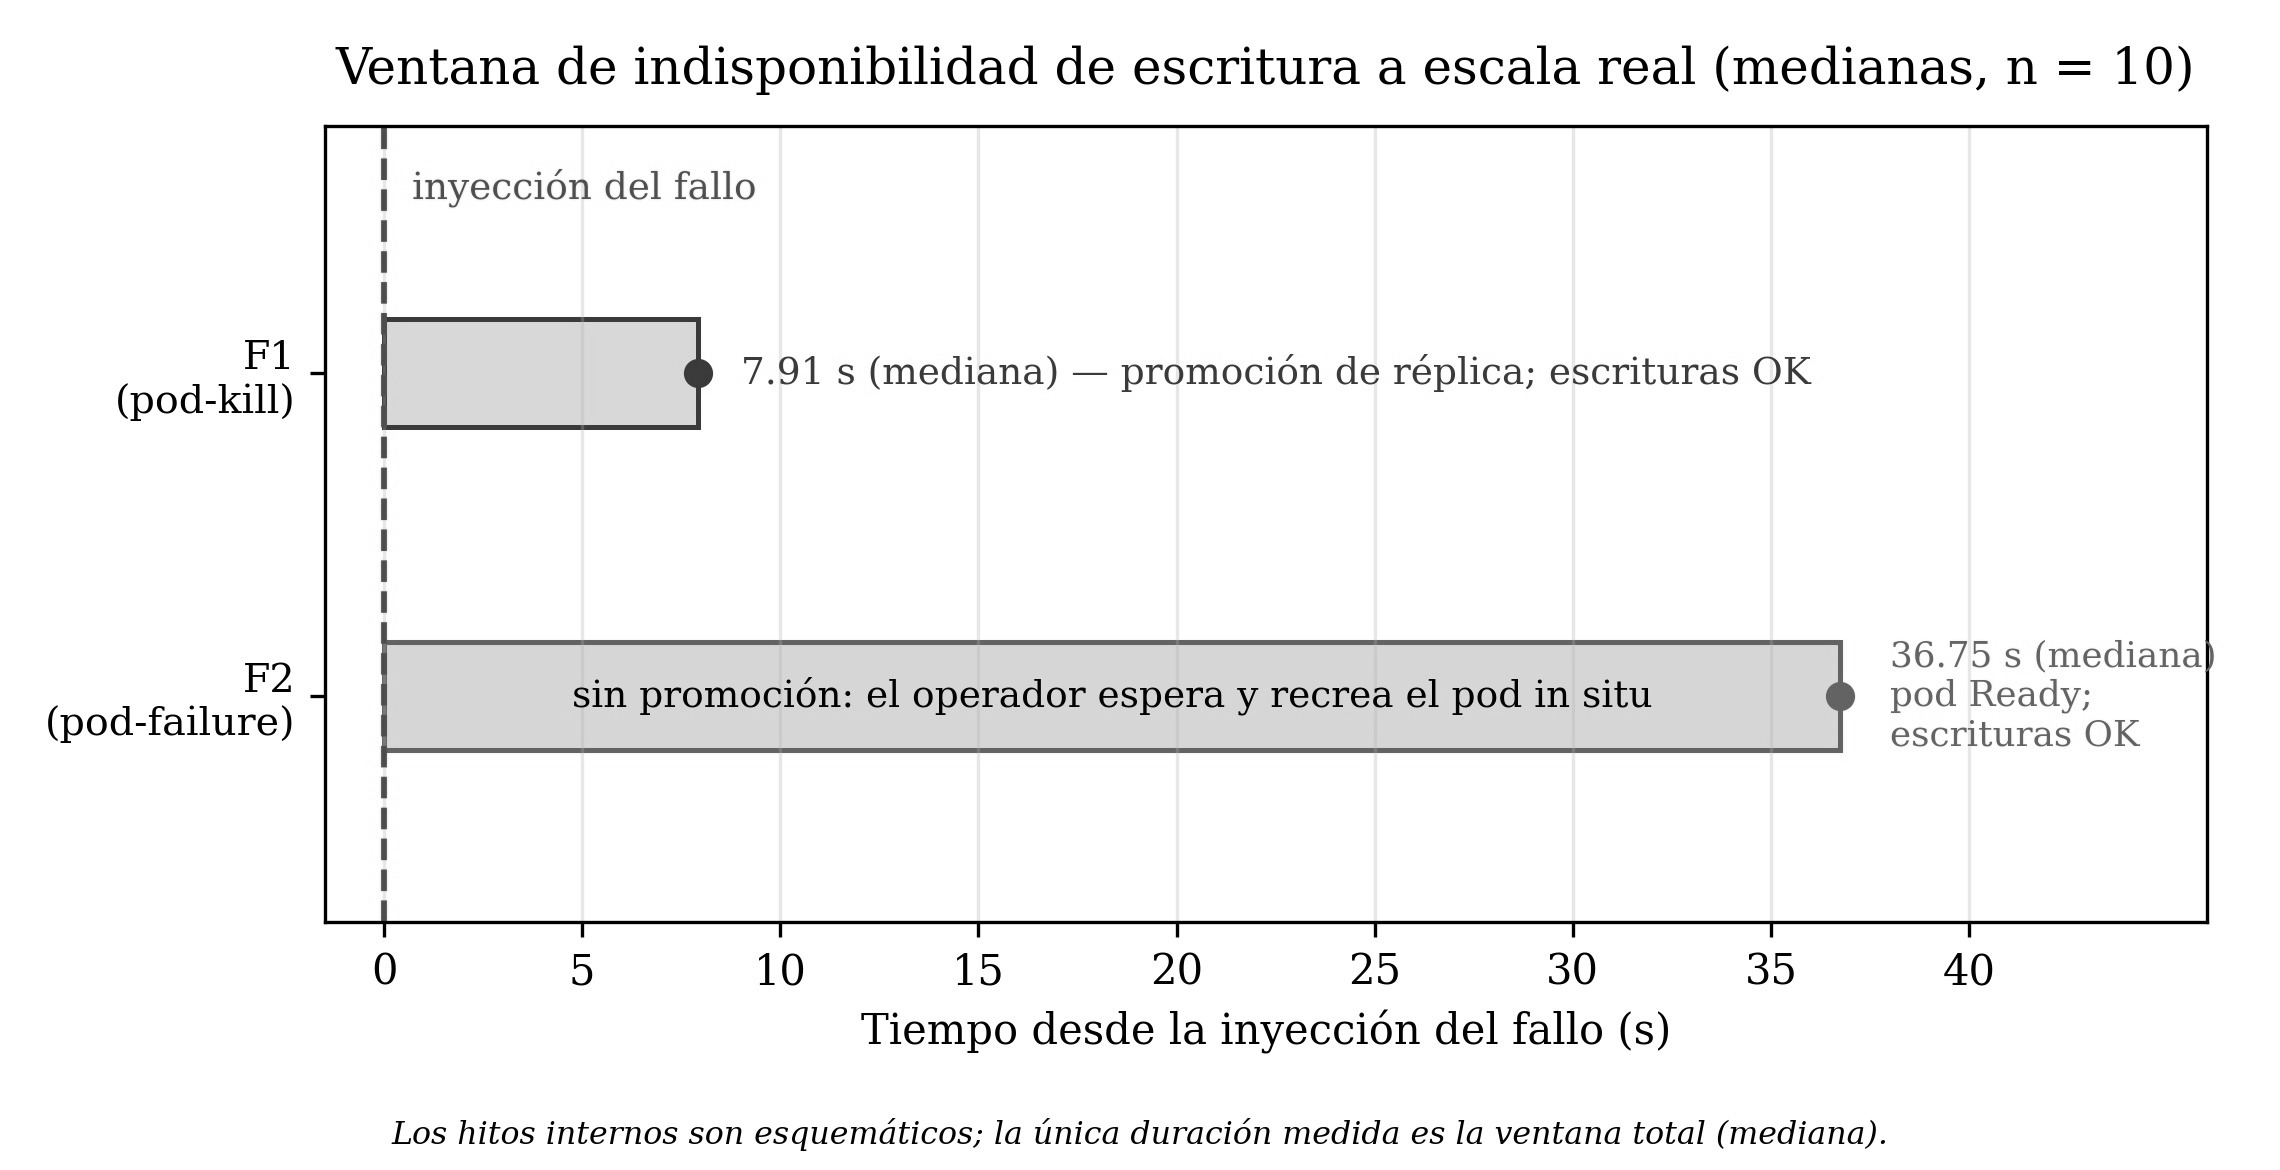
\includegraphics[width=0.92\textwidth]{figures/Fig4.jpg}
\caption{Ventana de indisponibilidad de escritura a escala real: F1 (7,91~s, promoción de réplica) frente a F2 (36,75~s, recreación in situ del pod). Fuente: mediciones del piloto.}
\label{fig:timeline}
\end{figure*}

La no promoción observada en F2 (0/10) y F3 (0/12) admite una cota superior por intervalo binomial exacto (Clopper--Pearson): la probabilidad real de promoción es $\le 25{,}9\%$ para 0/10 y $\le 22{,}1\%$ para 0/12 (cotas \emph{unilaterales} al 95\%; las bilaterales serían $30{,}8\%$ y $26{,}5\%$). No obstante, la conclusión de que estos escenarios no inducen promoción se apoya sobre todo en el mecanismo observado —CloudNativePG recrea el pod con la misma identidad y PVC, o mantiene \textit{Ready} al pod aislado— y no únicamente en el conteo.

El hallazgo central que articula estos tres comportamientos es que la variable que determina el \textit{failover} en CloudNativePG no es el fallo en sí, sino su visibilidad ante Kubernetes. En F1, la muerte del contenedor deja el pod en \textit{NotReady}; el operador registra el evento «\textit{Current primary isn't healthy, initiating a failover}» y promueve una réplica en $\approx 7{,}9$~s. En F3, las sondas del \textit{kubelet} no se bloquean —el \textit{failsafe} de Calico preserva el tráfico de \textit{host}—, de modo que el pod aislado permanece \textit{Ready}, el operador no emite evento alguno y no promueve: elige consistencia sobre disponibilidad (comportamiento CP) sin incurrir en \textit{split-brain}. F2 refina el mecanismo: aunque el pod queda \textit{NotReady}, se recrea con la misma identidad y el mismo PVC, y el operador prefiere esperar esa recreación en su sitio antes que promover. La promoción de F1 se explica, por tanto, por la eliminación del pod —el primario deja de existir— y no por el mero estado \textit{NotReady}.

\subsection{Sensibilidad a la latencia de E/S}
El escenario F4 —análisis de sensibilidad del RTO frente a niveles crecientes de latencia de E/S mediante IOChaos— resultó no ejecutable sobre CloudNativePG, y ese bloqueo constituye una lección de instrumentación. El inyector FUSE \texttt{toda} de Chaos Mesh realizó un \textit{ptrace attach} sobre el proceso de PostgreSQL, pero al intentar montar el sistema de archivos FUSE falló con \texttt{Read-only file system (os error 30)} y entró en un ciclo de reintentos. La causa es que CloudNativePG endurece sus pods con \texttt{readOnlyRootFilesystem: true} —junto con \texttt{runAsNonRoot} y el descarte de capacidades—, mientras que \texttt{toda} requiere un sistema de archivos raíz escribible para su andamiaje de montaje. La configuración del experimento era correcta: la verificación previa (\textit{dry-run}) de los selectores resolvió exclusivamente a los pods del clúster experimental y el recurso PodIOChaos se construyó con la ruta de volumen, el contenedor y los parámetros de latencia adecuados. No se trata, por tanto, de un error de configuración, sino de una incompatibilidad entre el inyector FUSE de Chaos Mesh y el \texttt{readOnlyRootFilesystem} de CloudNativePG.

Este resultado se registra estrictamente como una limitación de instrumentación observada con este par concreto de herramientas —el inyector FUSE de Chaos Mesh y el endurecimiento de CloudNativePG—, y no como una propiedad general de Chaos Mesh ni de los operadores. La medición cuantitativa de la sensibilidad a la latencia de E/S se asigna a la Fase~2. Dos vías la harían viable: un test confirmatorio que desactive \texttt{readOnlyRootFilesystem} para aislar la causa del bloqueo, y la limitación de ancho de banda de E/S a nivel de \textit{cgroup} (\texttt{io.max}), que no depende de FUSE ni requiere modificar el sistema bajo prueba.

\subsection{Contraste entre el comportamiento anticipado y el observado}
El vocabulario $S=(O,K,M,D)$ y la Tabla~\ref{tab:responsabilidad} anticipaban, a partir del comportamiento documentado, que el fallo del pod primario dispara la promoción de una réplica. El escenario F1 confirma esta expectativa —casi trivial—: el operador detecta la pérdida del líder y promueve, y el RTO observado resulta de la composición temporal de la detección, la promoción y el restablecimiento del enrutamiento. El aporte probatorio de mayor peso, sin embargo, no está en F1 sino en F2: la indisponibilidad sostenida del primario no promovió una réplica en ninguna de las diez repeticiones, en contra de la expectativa —derivada de tratar la indisponibilidad sostenida como aproximación de un fallo de nodo (Tabla~\ref{tab:responsabilidad}), que sí ordenaría promoción— de que se promovería una réplica. Un lector familiarizado con la semántica de \textit{pod-failure} podría anticipar la no-promoción; el aporte no es, pues, la sorpresa, sino la confirmación empírica y el aislamiento del mecanismo. Esta caracterización muestra que la promoción no depende del mero estado \textit{NotReady} del pod, sino de la pérdida de su identidad; cuando el pod se recrea con el mismo nombre y el mismo PVC, el operador prefiere esperar esa recreación en su sitio antes que promover. F3, por su parte, exhibe el comportamiento CP ante la partición de red —el operador evita el \textit{split-brain} apoyándose en el estado del \textit{API server}, como recoge la última fila de la Tabla~\ref{tab:responsabilidad}.

Los tres comportamientos comparten una misma variable de control que el marco actual no captura de forma explícita: la visibilidad del fallo ante Kubernetes (Fig.~\ref{fig:visibilidad}). De ahí que se proponga extender $S=(O,K,M,D)$ con un predicado de visibilidad $V(\text{fallo},K)$, según la \Ec{eq:visibilidad}, que registre el estado del pod primario ante el plano de control —eliminado (F1), \textit{NotReady}-recreado (F2) o \textit{Ready} (F3)— como la dimensión que ordena el gradiente de RTO observado:
\begin{equation}\label{eq:visibilidad}
\begin{aligned}
V(\text{fallo},K) \in \{\,&\text{eliminado},\ \text{NotReady-recreado},\\
&\text{Ready}\,\}.
\end{aligned}
\end{equation}
Se presenta como una extensión propuesta, motivada por la evidencia, y no como una relación derivada formalmente del marco. El bloqueo de F4 apunta a una segunda extensión pendiente: la observabilidad e \textit{inyectabilidad} de los fallos —y no solo su ocurrencia— dependen del endurecimiento del operador, una interacción que el modelo actual tampoco recoge. No se reclama, por tanto, una validación del marco, sino una caracterización empírica que lo confronta con el comportamiento observado y señala hacia dónde extenderlo.

\begin{figure}[tb]
\centering
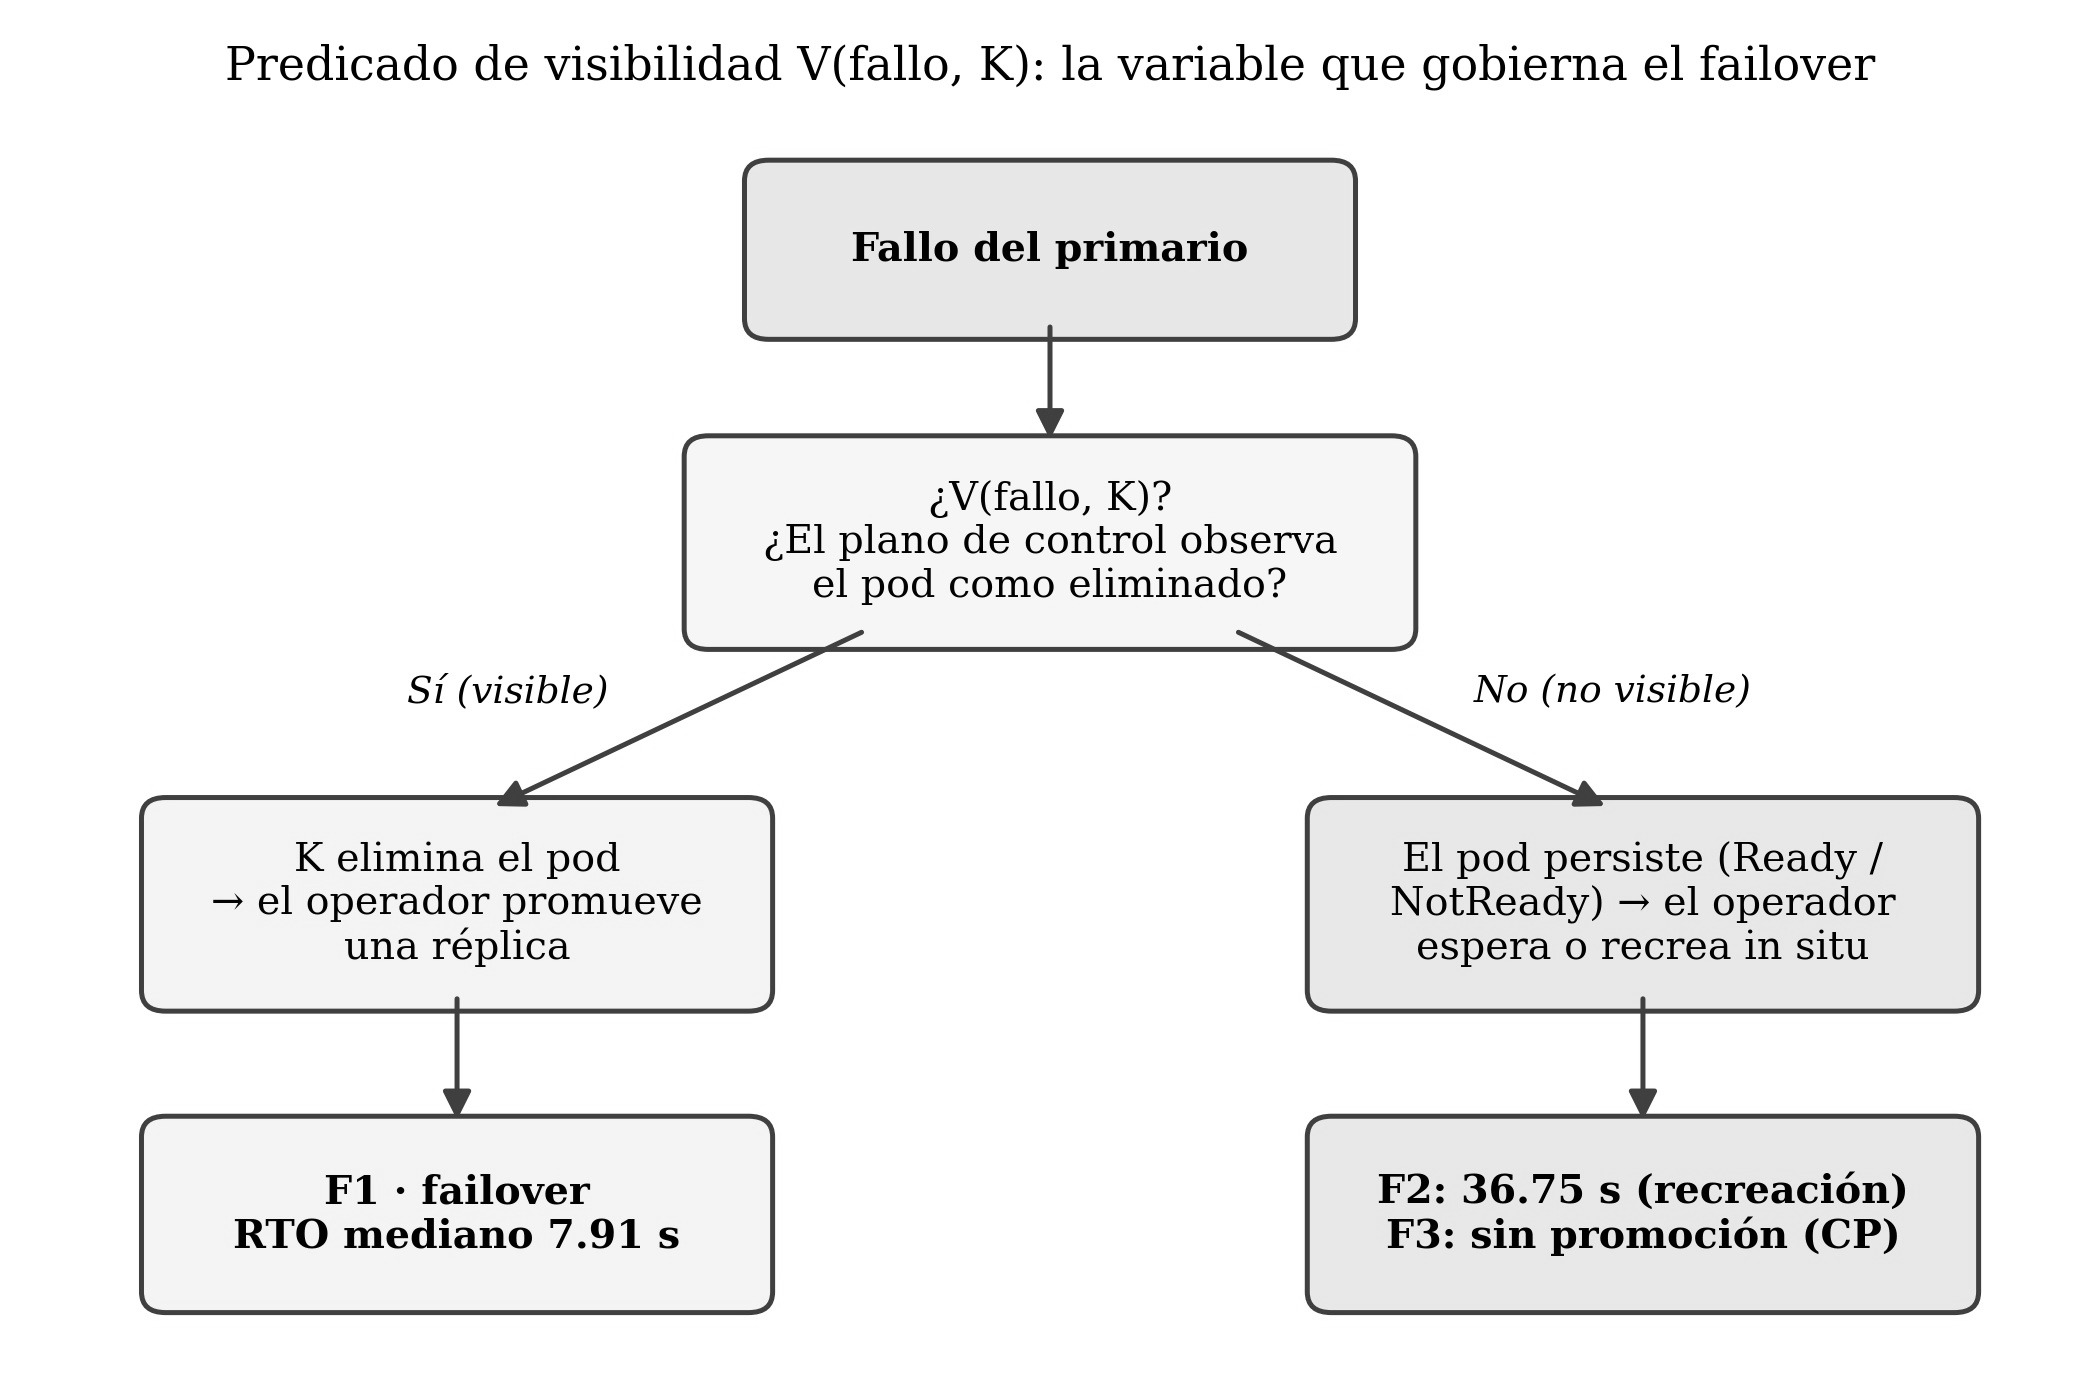
\includegraphics[width=\linewidth]{figures/Fig5.jpg}
\caption{Predicado de visibilidad $V(\text{fallo},K)$: la promoción se dispara solo cuando el plano de control observa el pod como eliminado (F1); si el pod persiste (F2, F3), el operador no promueve.}
\label{fig:visibilidad}
\end{figure}

Estos resultados se discuten en la Sección~7 a la luz de los invariantes definidos en la Sección~3.4.

\section{Discusión}
El comportamiento de sistemas PostgreSQL en Kubernetes no puede explicarse considerando una sola de sus capas: la interacción entre operador, almacenamiento y semántica de la base de datos introduce efectos emergentes que los enfoques centrados en un único componente no capturan. La confiabilidad en entornos \textit{cloud-native} es, por tanto, un fenómeno inherentemente multicapa, y decisiones aparentemente locales —la elección de operador o de tipo de almacenamiento— pueden tener implicaciones globales en métricas críticas como RTO, RPO o la visibilidad de las transacciones (Gilbert \& Lynch, 2002; Avizienis et al., 2004; Bailis \& Ghodsi, 2013). El modelo propuesto ofrece una base conceptual para analizar estas dependencias: la función de interacción multicapa $I(S)$ permite interpretar cómo la combinación de operador, almacenamiento y base de datos condiciona el comportamiento del sistema, extendiendo enfoques previos que los analizan por separado.

El alcance corresponde a una fase piloto (Fase~1) ejecutada dentro de las restricciones del entorno productivo (Sección~5). Tres limitaciones acotan la lectura de los resultados, ya detalladas en las Secciones~5 y~6: (i) se cubre un único operador (CloudNativePG) y una única categoría de almacenamiento —CSI en red—, por lo que la comparación entre operadores y categorías se aborda de forma analítica (Tabla~\ref{tab:responsabilidad}) y se asigna a la Fase~2; (ii) el fallo de nodo no se reprodujo —las tres instancias co-residieron en un único nodo—, de modo que el \textit{failover} observado es intra-nodo, la tolerancia a un fallo de nodo completo no fue \textit{testeable}, y tanto el RPO nulo de F1 como el RTO de F2 deben leerse como resultados acotados (este último, cota inferior del RTO real ante pérdida de nodo, al no capturar la latencia de reasociación \textit{detach/attach} del volumen CSI); y (iii) el análisis de sensibilidad a la E/S (F4) no fue ejecutable por la incompatibilidad entre el endurecimiento del operador (\texttt{readOnlyRootFilesystem}) y el inyector FUSE. Pese a ello, el trabajo aporta un marco que conecta distintas líneas de investigación y operacionaliza sus invariantes mediante métricas observables en un entorno productivo.

La Fase~2 —ya diseñada, con protocolo de ejecución e instrumentación desarrollados— ampliará la validación mediante un diseño factorial 2$\times$2 (replicación asíncrona frente a síncrona por quórum $\times$ topología co-localizada frente a anti-afinidad multi-nodo), incorporando los operadores y categorías de almacenamiento no cubiertos y un escenario de fallo de nodo genuino.

\section{Conclusiones}
Este trabajo abordó los sistemas PostgreSQL en Kubernetes desde una perspectiva multicapa, considerando conjuntamente la interacción entre operadores, almacenamiento basado en CSI y la semántica de la base de datos. Como contribución principal se presentó una taxonomía y un marco descriptivo —el vocabulario $S=(O,K,M,D)$ con sus invariantes— junto con un estudio empírico que lo confronta con el comportamiento observado mediante inyección controlada de fallos sobre un clúster productivo (Secciones~5 y~6), midiendo RTO, RPO y visibilidad de transacciones para CloudNativePG. El hallazgo central es que la variable que gobierna el \textit{failover} no es el fallo en sí, sino su visibilidad ante Kubernetes: la refutación de que la indisponibilidad sostenida del primario promovería una réplica —no lo hizo en ninguna de las diez repeticiones— es el resultado de mayor fuerza probatoria, y motiva extender el marco con un predicado de visibilidad $V(\text{fallo},K)$. La contribución conceptual de mayor alcance es, de hecho, ese predicado de visibilidad; la tupla $S=(O,K,M,D)$ actúa como andamiaje descriptivo que organiza el análisis, no como un modelo predictivo.

El análisis evidencia que la confiabilidad de cargas \textit{stateful} en Kubernetes no depende exclusivamente de la calidad de un operador o de las propiedades del almacenamiento, sino del comportamiento emergente de su interacción, con \textit{trade-offs} entre rendimiento, disponibilidad y consistencia que atraviesan múltiples capas. Ello subraya la necesidad de enfoques integrados de diseño y evaluación para arquitecturas \textit{cloud-native} donde la persistencia y la tolerancia a fallos son críticas.

El aporte de fondo es doble: el trabajo acerca la teoría de sistemas distribuidos a las implementaciones prácticas en Kubernetes y entrega una herramienta reutilizable —el modelo $S=(O,K,M,D)$ con sus invariantes operacionalizados— aplicable a otras configuraciones de operador y almacenamiento. Su validación se ampliará en la Fase~2 ya diseñada (Sección~7).

\section*{Agradecimientos}
Durante la preparación de este trabajo, el autor utilizó herramientas de inteligencia artificial generativa con el único fin de mejorar la redacción, la gramática, la concisión y el estilo del manuscrito. La concepción de la investigación, el modelo formal, la ejecución experimental, el análisis y las conclusiones son obra exclusiva del autor, quien revisó y validó la totalidad del contenido y asume la plena responsabilidad por su exactitud, originalidad e integridad. El autor único realizó la conceptualización, la metodología, la ejecución experimental, el análisis y la redacción del manuscrito. Esta investigación no recibió financiamiento externo y el autor declara no tener ningún conflicto de interés. Los datos limpios de RTO/RPO por escenario y el paquete de ejecución —manifiestos del clúster y de Chaos Mesh, el cliente verificador de transacciones, la carga pgbench y los scripts de análisis— se depositan públicamente en Zenodo (DOI por asignar). Los registros crudos del verificador y los eventos del operador se facilitan a petición, ya que el experimento se ejecutó sobre un clúster productivo bajo acceso restringido; el material depositado permite reproducir el diseño en un clúster equivalente.

% ============================================================================
%  BIBLIOGRAFÍA — orden alfabético, formato Faraute (autor. año. título...)
% ============================================================================
\phantomsection
\section*{Referencias}
\begingroup
\footnotesize
\setlength{\parindent}{-1.2em}
\setlength{\leftskip}{1.2em}
\setlength{\parskip}{4pt}

Alquraan, A., H. Takruri, M. Alfatafta \& S. Al-Kiswany. (2018). An analysis of network-partitioning failures in cloud systems. \textit{Proc. 13th USENIX Symp. Operating Systems Design and Implementation (OSDI 18)}. USENIX Association. Carlsbad, CA, USA. pp. 51--68.\par
Alvaro, P. \& S. Tymon. (2018). Abstracting the geniuses away from failure testing. \textit{Communications of the ACM} 61(1): 54--61.\par
Avizienis, A., J.-C. Laprie, B. Randell \& C. Landwehr. (2004). Basic concepts and taxonomy of dependable and secure computing. \textit{IEEE Trans. Dependable and Secure Computing} 1(1): 11--33.\par
Bailis, P. \& A. Ghodsi. (2013). Eventual consistency today: limitations, extensions, and beyond. \textit{Communications of the ACM} 56(5): 55--63.\par
Basiri, A., N. Behnam, R. de Rooij, L. Hochstein, L. Kosewski, J. Reynolds \& C. Rosenthal. (2016). Chaos engineering. \textit{IEEE Software} 33(3): 35--41.\par
Burckhardt, S. (2014). Principles of eventual consistency. \textit{Foundations and Trends in Programming Languages} 1(1--2): 1--150.\par
Burns, B., B. Grant, D. Oppenheimer, E. Brewer \& J. Wilkes. (2016). Borg, Omega, and Kubernetes. \textit{ACM Queue} 14(1): 70--93.\par
Chen, Z., M. Goudarzi \& A. N. Toosi. (2025). Resilience evaluation of Kubernetes in cloud-edge environments via failure injection. \textit{arXiv:2507.16109 [cs.DC]}.\par
CloudNativePG. (2026). CloudNativePG documentation. [En línea]. Disponible: \url{https://cloudnative-pg.io/docs/} [Consultado: 7 de julio de 2026].\par
Crunchy Data. (2026). PGO: the Postgres Operator from Crunchy Data --- documentation. [En línea]. Disponible: \url{https://access.crunchydata.com/documentation/postgres-operator/latest/} [Consultado: 7 de julio de 2026].\par
Dobies, J. \& J. Wood. (2020). \textit{Kubernetes Operators: automating the container orchestration platform}. O'Reilly Media. Sebastopol, CA, USA.\par
Drees, F. (2026). Chaos testing the CloudNativePG project. \textit{CloudNativePG Blog}. [En línea]. Disponible: \url{https://cloudnative-pg.io/blog/lfx-chaos-testing-yash-agarwal/} [Consultado: 8 de julio de 2026].\par
Gilbert, S. \& N. Lynch. (2002). Brewer's conjecture and the feasibility of consistent, available, partition-tolerant web services. \textit{ACM SIGACT News} 33(2): 51--59.\par
Han, F. et al. (2024). PALF: replicated write-ahead logging for distributed databases. \textit{Proc. VLDB Endowment} 17(12): 3745--3758.\par
Khan, W., T. Kumar, C. Zhang, K. Raj, A. M. Roy \& B. Luo. (2023). SQL and NoSQL database software architecture performance analysis and assessments --- a systematic literature review. \textit{Big Data and Cognitive Computing} 7(2): art. 97.\par
Kingsbury, K. \& P. Alvaro. (2021). Elle: inferring isolation anomalies from experimental observations. \textit{Proc. VLDB Endowment} 14(3): 268--280.\par
Kubernetes. (2024). Container storage interface (CSI). \textit{Kubernetes Documentation}. [En línea]. Disponible: \url{https://kubernetes.io/docs/concepts/storage/volumes/} y la especificación versionada en \url{https://github.com/container-storage-interface/spec} [Consultado: 2024].\par
Kubernetes. (2026a). Nodes: node controller, condiciones del nodo y desalojo basado en taints. \textit{Kubernetes Documentation}. [En línea]. Disponible: \url{https://kubernetes.io/docs/concepts/architecture/nodes/} [Consultado: 7 de julio de 2026].\par
Kubernetes. (2026b). Operator pattern. \textit{Kubernetes Documentation}. [En línea]. Disponible: \url{https://kubernetes.io/docs/concepts/extend-kubernetes/operator/} [Consultado: 8 de julio de 2026].\par
Mega, C. (2023). Orchestrating information governance workloads as stateful services using Kubernetes operator framework. \textit{Service-Oriented Computing (SummerSOC 2023), Communications in Computer and Information Science}, vol. 1847. Springer. Cham, Switzerland. pp. 125--143.\par
Ongaro, D. \& J. Ousterhout. (2014). In search of an understandable consensus algorithm (Raft). \textit{Proc. USENIX Annual Technical Conf. (USENIX ATC)}. USENIX Association. pp. 305--319.\par
Patroni. (2026). Patroni: a template for PostgreSQL HA with ZooKeeper, etcd or Consul --- documentation. [En línea]. Disponible: \url{https://patroni.readthedocs.io/} [Consultado: 7 de julio de 2026].\par
Portworx. (s.f.). Choosing a Kubernetes operator for PostgreSQL. [En línea]. Disponible: \url{https://portworx.com/blog/choosing-a-kubernetes-operator-for-postgresql/}.\par
PostgreSQL Global Development Group. (2024). PostgreSQL 16 documentation: streaming replication y \texttt{synchronous\_commit}. [En línea]. Disponible: \url{https://www.postgresql.org/docs/16/} [Consultado: 2024].\par
Schwarzkopf, M., A. Konwinski, M. Abd-El-Malek \& J. Wilkes. (2013). Omega: flexible, scalable schedulers for large compute clusters. \textit{Proc. EuroSys}. ACM. pp. 351--364.\par
simplyblock. (s.f.). How to choose your Kubernetes Postgres operator? [En línea]. Disponible: \url{https://simplyblock.io/blog/choosing-a-kubernetes-postgres-operator/}.\par
Stonebraker, M. \& G. Kemnitz. (1991). The POSTGRES next-generation database management system. \textit{Communications of the ACM} 34(10): 78--92.\par
Taft, R. et al. (2020). CockroachDB: the resilient geo-distributed SQL database. \textit{Proc. ACM SIGMOD Int. Conf. Management of Data}. ACM. pp. 1493--1509.\par
van Renesse, R. \& F. B. Schneider. (2004). Chain replication for supporting high throughput and availability. \textit{Proc. OSDI}. USENIX Association.\par
\endgroup

\end{document}
